% ============================================================
% BÖLÜM 3 - INNATE MİMARİSİ VE YÖNTEM
% ============================================================
\chapter{INNATE MİMARİSİ VE YÖNTEM}
\label{ch:mimari}

\section{Hesaplama Bölgesi ve Parametreler}
\label{sec:hesaplama_bolgesi}

Bu çalışmada hesaplama bölgesi $\Omega = [0,L_{x}]\times[0,L_{y}]\times[0,L_{z}]$ üç boyutlu kutu olarak alınmış, ızgara $N_{x}\times N_{y}\times N_{z} = 96\times 160\times 64$ olarak yapılandırılmıştır. Boyutlar dikey eksen $y$ yönünde uzatılmış, $L_{x}=6$, $L_{y}=10$, $L_{z}=4$ olarak seçilmiştir. Bu seçim, kaldırma kuvvetinin uygulandığı dikey yönde yeterli çözünürlük sağlamak ve aynı zamanda yatay yönlerde periyodik tekrarlanma boyunu makul tutmak amacıyla yapılmıştır. Tüm yönlerde periyodik sınır koşulları geçerlidir.

Termal alan konvansiyonu şu şekildedir: $y=0$ alt sınırı sıcak ($T_{\mathrm{hot}}=20$), $y=L_{y}$ üst sınırı soğuk ($T_{\mathrm{cold}}=0$) olarak tanımlanmıştır. Doğrusal baz profil $T_{\mathrm{base}}(y) = T_{\mathrm{hot}} - (T_{\mathrm{hot}}-T_{\mathrm{cold}})\,y/L_{y}$ olarak verilir; bu, $\partial T_{\mathrm{base}}/\partial y = -\Delta T/L_{y}$ negatif gradyenine karşılık gelir. Bu konvansiyon, alttan ısıtılan, üstten soğutulan bir konfigürasyon olup Rayleigh--B\'enard benzeri kaldırma-kararsız bir karakter sergiler. Sıcaklık dalgalanması $\theta(\mathbf{x},t) = T(\mathbf{x},t) - T_{\mathrm{base}}(y)$ olarak tanımlanır ve enerji denklemine $S_{\theta} = +v/L_{y}$ kaynak terimi olarak girer; bu terim, sıcak parçacıkların yukarı çıkarken daha soğuk baz tabakaya girmesiyle $\theta$'nın artmasını fiziksel olarak ifade eder.

Boyutsuz parametreler $\mathrm{Re}\in\{7000,10\,000\}$, $\mathrm{Ra}=10^{5}$, $\mathrm{Pr}=0.71$ olarak alınmış; karşılık gelen Richardson sayısı $\mathrm{Ri}\approx 1.4\times 10^{-3}$ olup zorlanmış konveksiyon baskın, hafif-kaldırmalı bir rejimi belirler. Büyük ölçek zorlaması Kolmogorov tipi olup $k_{f}=4$ dalga sayısında uygulanır; bu, yatay düzlemde dört adet karşıt-dönen hücre üreterek türbülans kademesini başlatır. Zaman adımı $\Delta t = 0.02$, toplam katman sayısı $N_{\mathrm{layer}}=20$ olup her bir katman tek bir fraksiyonel adım IMEX zaman ilerletmesini temsil eder; bu durumda tek bir ileri geçiş $20\Delta t = 0.4$ birim zaman ilerletir.

Hesaplama bölgesinin şematik gösterimi, Kolmogorov forcing'in uygulandığı $k_{f}=4$ moduyla birlikte Şekil~\ref{fig:domain_schema}'da verilmiştir.

\begin{figure}[H]
\centering
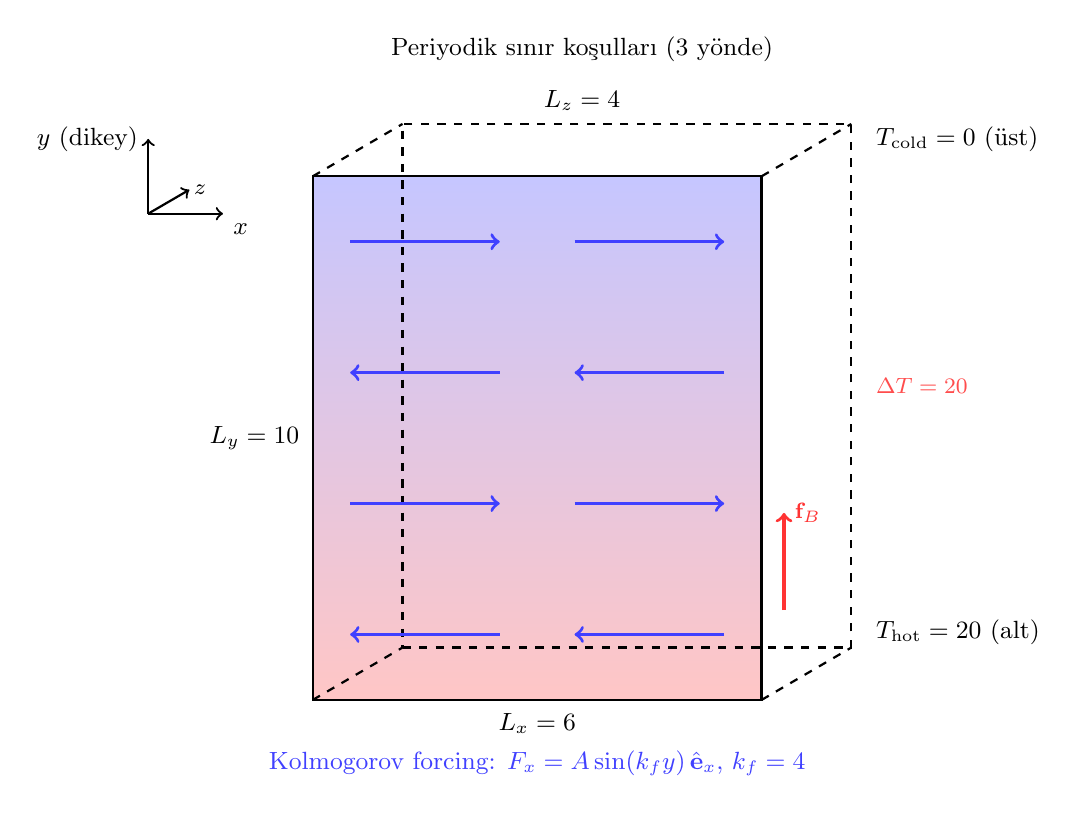
\begin{tikzpicture}[scale=0.95]
  % 3D perspektif kutu — y dikey, x yatay, z derinlik
  % Ön yüz: x-y düzlemi (0,0) (6,0) (6,7) (0,7)  [y skala = 7]
  % Z derinlik perspektif ofseti (z_proj_x, z_proj_y) = (1.2, 0.7)
  \def\zx{1.2}\def\zy{0.7}
  % Ön yüz dolgu (sıcaklık gradyanı)
  \shade[bottom color=red!50, top color=blue!50, opacity=0.45] (0,0) rectangle (6,7);
  % Ön yüz kenarları
  \draw[thick] (0,0) -- (6,0) -- (6,7) -- (0,7) -- cycle;
  % Arka yüz kenarları (kesikli)
  \draw[thick, dashed] (\zx,\zy) -- (6+\zx,\zy) -- (6+\zx,7+\zy) -- (\zx,7+\zy) -- cycle;
  % Bağlantı kenarları
  \draw[thick, dashed] (0,0) -- (\zx,\zy);
  \draw[thick, dashed] (6,0) -- (6+\zx,\zy);
  \draw[thick, dashed] (0,7) -- (\zx,7+\zy);
  \draw[thick, dashed] (6,7) -- (6+\zx,7+\zy);

  % Eksen takımı (sol-üst köşede, Kolmogorov yazısı ile çakışmasın)
  \begin{scope}[shift={(-2.2, 6.5)}]
    \draw[->, thick] (0,0) -- (1.0,0) node[below right, font=\small]{$x$};
    \draw[->, thick] (0,0) -- (0,1.0) node[left, font=\small]{$y$ (dikey)};
    \draw[->, thick] (0,0) -- (0.55,0.32) node[right, font=\footnotesize, xshift=-2pt]{$z$};
  \end{scope}

  % Boyut etiketleri (kutu etrafında, çakışmasız)
  \node[below, font=\small] at (3,-0.05) {$L_{x}=6$};
  \node[left, font=\small] at (-0.05,3.5) {$L_{y}=10$};
  % L_z etiketini arka-üst kenarın üstüne taşı (T_hot ile çakışmasın)
  \node[above, font=\small] at (3+\zx/2, 7+\zy+0.05) {$L_{z}=4$};

  % Sıcaklık etiketleri (sağ tarafta)
  \node[right, font=\small] at (6+\zx+0.2, \zy+0.2) {$T_{\mathrm{hot}}=20$\ (alt)};
  \node[right, font=\small] at (6+\zx+0.2, 7+\zy-0.2) {$T_{\mathrm{cold}}=0$\ (üst)};
  \node[right, font=\footnotesize, color=red!70] at (6+\zx+0.2, 3.5+\zy) {$\Delta T = 20$};
  % Kaldırma kuvveti oku (yukarı, sıcak akışkan)
  \draw[->, thick, red!80, line width=1.2pt] (6.3, 1.2) -- (6.3, 2.5) node[right, font=\footnotesize]{$\mathbf{f}_{B}$};

  % Kolmogorov forcing: F_x = A sin(k_f y) ê_x
  % y yükseldikçe yön x-yatay değişen, dört "karşıt-dönen" hücre
  % k_f = 4 → y boyunca 4 yarım-periyot, yani 2 tam periyot
  \foreach \i/\sign in {0.875/1, 2.625/-1, 4.375/1, 6.125/-1} {
    \draw[->, very thick, blue!75]
      (1.5+\sign*1.0,\i) -- (1.5-\sign*1.0,\i);
    \draw[->, very thick, blue!75]
      (4.5+\sign*1.0,\i) -- (4.5-\sign*1.0,\i);
  }

  % Başlık etiketleri
  \node[above, font=\small] at (3.6, 7+\zy+0.7) {Periyodik sınır koşulları (3 yönde)};
  \node[below, font=\small, blue!75] at (3, -0.55) {Kolmogorov forcing: $F_{x} = A\sin(k_{f}y)\,\hat{\mathbf{e}}_{x}$, $k_{f}=4$};
\end{tikzpicture}
\caption{Hesaplama bölgesi, sıcaklık baz profili ve $k_{f}=4$ Kolmogorov zorlamasının şematik gösterimi. Dikey eksen $y$, $L_{y}=10$ ile en uzun yöndür ($96\times 160\times 64$ ızgarada en yüksek çözünürlüğe sahiptir). Kolmogorov zorlaması $x$-bileşeninde olup $y$ boyunca işaret değiştirir (oklar). Sıcak alt sınır kaldırma kuvveti $\mathbf{f}_{B}=\mathrm{Ri}\,\theta\,\hat{\mathbf{e}}_{y}$'yi (kırmızı ok) yukarı yönde üretir.}
\label{fig:domain_schema}
\end{figure}

Çalışmanın merkezi konfigürasyon parametreleri Kod~\ref{code:config}'te \texttt{config.py} dosyasının özet biçimi olarak verilmiştir.

\begin{lstlisting}[caption={Konfigürasyon dataclass'ları (özet). Tam dosya: \texttt{config.py}.}, label={code:config}]
@dataclass
class DomainConfig:
    Lx: float = 6.0;   Ly: float = 10.0;  Lz: float = 4.0
    Nx: int   = 96;    Ny: int   = 160;   Nz: int   = 64

@dataclass
class PhysicsConfig:
    Re: float = 10000.0
    Ra: float = 1e5
    Pr: float = 0.71
    dt: float = 0.020
    T_hot: float = 20.0   # y = 0 (alt sınır)
    T_cold: float = 0.0   # y = L_y (üst sınır)
    forcing_mode: str = "kolmogorov"
    k_f: int = 4

    @property
    def nu(self):    return 1.0 / self.Re
    @property
    def kappa(self): return 1.0 / (self.Re * self.Pr)
    @property
    def Ri(self):    return self.Ra / (self.Re ** 2 * self.Pr)

@dataclass
class ModelConfig:
    n_layers: int = 20
    use_eddy_viscosity: bool = True
    use_anisotropic_sgs: bool = True
    use_per_layer_buoyancy: bool = True
    use_per_layer_dt: bool = True
    use_imex: bool = True
    use_spectral_cs: bool = True      # Spectral-Cs v3 (MLP YOK)
    spectral_cs_kx_max: int = 5
    spectral_cs_ky_max: int = 8
    spectral_cs_kz_max: int = 6

@dataclass
class TrainingConfig:
    lr: float = 3e-4
    weight_decay: float = 0.0          # MLP yok, weight decay zararlı
    warmup_epochs: int = 100
    max_epochs: int = 1500
    grad_clip: float = 5.0
    freeze_canonical_params: bool = True   # Tier 1 hijyen
\end{lstlisting}

\section{Saf-Fizik Nöron Kütüphanesi}

INNATE'in çekirdek prensibi, fiziksel operatörlerin doğrudan ağı oluşturan nöronlar olarak tanımlanmasıdır. Bu bölümde her bir nöron tipinin matematiksel formülasyonu, içerdiği öğrenilebilir parametreler ve uygulama detayları sunulmaktadır.

\subsection{Adveksiyon Nöronu (Advection3D)}

Momentum adveksiyonu, kinetik enerjinin sürekli zamanda L²-integralinde korunduğu \emph{rotasyonel (Lamb) form}da yazılır \cite{morinishi_skew_1998}:
\begin{equation}
\mathcal{N}_{\mathrm{adv}}(\mathbf{u}) = (\mathbf{u}\cdot\nabla)\mathbf{u}
= \boldsymbol{\omega}\times\mathbf{u} + \nabla\!\left(\tfrac{1}{2}|\mathbf{u}|^{2}\right),
\label{eq:advection_lamb}
\end{equation}
burada $\boldsymbol{\omega}=\nabla\times\mathbf{u}$ vortisitedir. Lamb formunun en önemli özelliği, dinamik basınç terimi $\nabla(\tfrac{1}{2}|\mathbf{u}|^{2})$'nin Leray (Helmholtz) projeksiyonu tarafından otomatik olarak ayrıştırılıp basınca gömülmesidir; dolayısıyla diverjans-serbest hız alanı için $\mathbf{u}\cdot\boldsymbol{\omega}\times\mathbf{u}=0$ vektör özdeşliği gereği toplam kinetik enerjiye katkı L²-integralinde sıfırdır. Bu yapı, ayrık zamanda da konvektif veya divergence formuna kıyasla enerji drift'ini belirgin biçimde sınırlar. Bunun bir alternatifi olarak \emph{skew-simetrik form} ($\tfrac{1}{2}[(\mathbf{u}\cdot\nabla)\mathbf{u}+\nabla\cdot(\mathbf{u}\otimes\mathbf{u})]$) da uygulanabilir; bu çalışmada varsayılan olarak Lamb formu seçilmiştir.

Kod~\ref{code:advection}'da \texttt{Advection3D} nöronunun forward fonksiyonu özetlenmiştir. Üretilen tensör çıktıları (\texttt{adv\_u}, \texttt{adv\_v}, \texttt{adv\_w}) sonradan IMEX zaman ilerletmesi içinde sağ-taraf (RHS) terimine eklenir.

\begin{lstlisting}[caption={\texttt{Advection3D} nöronu: varsayılan Lamb form (\texttt{use\_lamb=True}); skew-simetrik form alternatif olarak mevcuttur. Tam dosya: \texttt{innate.py:2520+}.}, label={code:advection}]
class Advection3D(nn.Module):
    """3D Adveksiyon Nöronu: (u . grad) u  = omega x u + grad(|u|^2/2)
    TEK NÖRON = TEK FİZİKSEL OPERATÖR
    """
    def __init__(self, resolution, diff_ops, use_lamb=True):
        super().__init__()
        self.diff_ops = diff_ops
        self.use_lamb = use_lamb        # varsayılan: True (Lamb form)
        # TEK ÖĞRENİLEBİLİR PARAMETRE
        self.advection_modulator = nn.Parameter(torch.ones(1))

    def forward(self, state, vel_grads=None):
        u, v, w = state.u, state.v, state.w
        ops = self.diff_ops

        if self.use_lamb:
            # Lamb form: omega x u  (grad(|u|^2/2) basinca gomulur, Leray projection)
            omega_x, omega_y, omega_z = ops.curl(u, v, w)
            adv_u = omega_y * w - omega_z * v
            adv_v = omega_z * u - omega_x * w
            adv_w = omega_x * v - omega_y * u
        else:
            # Skew-symmetric form (alternatif): 0.5*(convective + divergence)
            if vel_grads is None:
                du = ops.gradient(u);  dv = ops.gradient(v);  dw = ops.gradient(w)
            else:
                du, dv, dw = vel_grads[0:3], vel_grads[3:6], vel_grads[6:9]
            adv_u_c = u*du[0] + v*du[1] + w*du[2]
            adv_v_c = u*dv[0] + v*dv[1] + w*dv[2]
            adv_w_c = u*dw[0] + v*dw[1] + w*dw[2]
            uu, vv, ww = ops.dealias(u*u), ops.dealias(v*v), ops.dealias(w*w)
            uv, uw, vw = ops.dealias(u*v), ops.dealias(u*w), ops.dealias(v*w)
            adv_u_d, _, _ = ops.div_tensor((uu, uv, uw))
            _, adv_v_d, _ = ops.div_tensor((uv, vv, vw))
            _, _, adv_w_d = ops.div_tensor((uw, vw, ww))
            adv_u = 0.5 * (adv_u_c + adv_u_d)
            adv_v = 0.5 * (adv_v_c + adv_v_d)
            adv_w = 0.5 * (adv_w_c + adv_w_d)

        # Parametre kacisini sinirla: 0.5 <= mod <= 1.5
        mod = torch.clamp(self.advection_modulator, 0.5, 1.5)
        return mod * adv_u, mod * adv_v, mod * adv_w
\end{lstlisting}

Adveksiyon nöronunun tek bir öğrenilebilir parametresi vardır: $\alpha_{\mathrm{adv}}^{(\ell)} \in \mathbb{R}$ katman-spesifik adveksiyon ölçekleme katsayısı. Parametre kaçışını sınırlamak için bu katsayı $[0.5, 1.5]$ aralığında \texttt{clamp} ile sınırlandırılmıştır. Toplam katkı $\alpha_{\mathrm{adv}}^{(\ell)}\,\mathcal{N}_{\mathrm{adv}}(\mathbf{u})$ olarak hesaplanır. Bu parametre, kanonik Boussinesq--Newton denklem yapısında $\alpha_{\mathrm{adv}}=1$ olmalıdır; ancak ön eğitim aşamasında modelin bu parametreyi öğrenilebilir bırakması, modelin denklemleri yeniden öğrenmesi (\textit{equation forgetting}) gibi anti-fiziksel davranışlara yol açmıştır (Bölüm~\ref{ch:bulgular}, Kademe~1 tartışması). Sonuç olarak çalışmanın final konfigürasyonunda bu parametre $\alpha_{\mathrm{adv}}^{(\ell)} = 1.0$ olarak dondurulmuştur. Adveksiyon nöronunun türev operatörleri Fourier uzayında çalışan paylaşımlı bir spektral operatör modülü (\texttt{SpectralOps3DAniso}) üzerinden hesaplanır.

\subsection{Difüzyon Nöronu}

Moleküler viskoz difüzyon $\nu\,\nabla^{2}\mathbf{u}$ Fourier uzayında doğrudan çarpım olarak hesaplanır:
\begin{equation}
\widehat{\nu\,\nabla^{2}\mathbf{u}}(\mathbf{k}) = -\nu\,|\mathbf{k}|^{2}\,\hat{\mathbf{u}}(\mathbf{k}).
\label{eq:diffusion_fourier}
\end{equation}
Bu nöron, IMEX (yarı örtük) entegrasyon nedeniyle açık biçimde bir kayıp olarak değil, zaman ilerletme denkleminin paydasında yer alır; ayrıntısı Bölüm~\ref{sec:imex_integrator}'de verilmiştir. Bu nedenle difüzyon nöronu hiçbir öğrenilebilir parametre içermez.

\subsection{Projeksiyon Nöronu (Projection3D)}

Sıkıştırılamazlık koşulu $\nabla\cdot\mathbf{u}=0$ her zaman adımı sonunda Helmholtz ayrışımı ile sağlanır. Spektral uzayda projeksiyon operatörü
\begin{equation}
\widehat{\mathbf{u}}^{\mathrm{div\text{-}free}}(\mathbf{k})
= \left(I - \frac{\mathbf{k}\otimes\mathbf{k}}{|\mathbf{k}|^{2}}\right)\hat{\mathbf{u}}(\mathbf{k}),
\quad \widehat{\mathbf{u}}^{\mathrm{div\text{-}free}}(\mathbf{0}) = 0,
\label{eq:projection}
\end{equation}
biçimindedir. Bu operatör, çıktısı diverjans-serbest olduğu için $\nabla\cdot\mathbf{u}=0$ koşulunu \emph{yapısal} olarak garanti eder. Projeksiyon nöronu hiçbir öğrenilebilir parametre içermez.

\subsection{Termal Adveksiyon ve Difüzyon Nöronları}

Sıcaklık dalgalanması $\theta$ için adveksiyon nöronu, momentum adveksiyonunun aksine non-konservatif formda yazılır (skaler alan için bu doğal seçim olduğu için):
\begin{equation}
\mathcal{N}_{\mathrm{th\text{-}adv}}(\mathbf{u},\theta) = (\mathbf{u}\cdot\nabla)\theta.
\label{eq:thermal_advection}
\end{equation}
Termal difüzyon nöronu $\kappa\,\nabla^{2}\theta$ benzer şekilde Fourier uzayında çarpım olarak hesaplanır; $\kappa = 1/(\mathrm{Re}\,\mathrm{Pr})$. Termal nöronların her ikisi de katman başına bir öğrenilebilir modülatör parametresi içerir; bu parametreler de Kademe~1 freeze politikası altında kanonik değerlerde sabitlenmiştir.

\subsection{Kaldırma Kuvveti Nöronu (Buoyancy3D)}

Boussinesq kaldırma terimi,
\begin{equation}
\mathbf{f}_{B}^{(\ell)}(\theta) = \mathrm{Ri}\,\beta_{B}^{(\ell)}\,\theta\,\hat{\mathbf{e}}_{y},
\label{eq:buoyancy_neuron}
\end{equation}
biçiminde uygulanır; burada $\beta_{B}^{(\ell)}$ katman başına ölçekleme parametresidir. Kanonik Boussinesq formunda $\beta_{B}=1$ olmalıdır. Ön çalışmalarda bu parametrenin öğrenilebilir bırakılması, modelin kaldırma kuvvetini abartmaya veya bastırmaya yönelmesine ve sonuç olarak anti-fiziksel Nusselt sayılarına yol açmıştır. Final konfigürasyonda $\beta_{B}^{(\ell)}=1.0$ olarak dondurulmuştur.

\subsection{Alt-Izgara Viskozite Nöronu (EddyViscosity3D)}
\label{subsec:eddy_viscosity}

Smagorinsky tipi alt-ızgara modeli denklem~\eqref{eq:smagorinsky}'deki gibi uygulanır, ancak Smagorinsky sabiti $C_{s}$ tek bir skaler olarak değil, uzaysal olarak değişen bir alan $C_{s}(\mathbf{x},t)$ olarak modellenmektedir. Bu alan, ön bölümde değinilen \emph{Spectral-Cs v3} parametrizasyonu (Bölüm~\ref{sec:spectral_cs}) ile temsil edilir.

Eddy viskozitesi nöronu, klasik Smagorinsky uygulamasının ötesinde iki ek özellik içerir:

\paragraph{Anizotropik SGS.} Yatay ve dikey gerinim bileşenleri farklı $C_{s}$ etkili değerleri ile çarpılarak anizotropik bir alt-ızgara modeli oluşturulur. Bu, dikey yönde kaldırma kuvvetinin neden olduğu farklı kademe dinamiklerini hesaba katar.

\paragraph{Türbülanslı Prandtl sayısı.} Termal alt-ızgara difüzivitesi denklem~\eqref{eq:turbulent_prandtl}'deki gibi $\alpha_{t} = \nu_{t}/\mathrm{Pr}_{t}$ olarak tanımlanır, ancak $\mathrm{Pr}_{t}$ sabit alınmaz: katman-bazında öğrenilebilir bir parametredir ($\mathrm{Pr}_{t}^{(\ell)}$, başlangıç değeri $0.85$). Bu, termal alanın momentum alanından ne ölçüde \emph{ayrıştığını} öğrenilen bir biçimde modellenmesine olanak sağlar.

\paragraph{Geri-saçılma (backscatter).} Eddy viskozitesi yalnızca pozitif değerler almaz; küçük negatif değerler, küçük ölçeklerden büyük ölçeklere enerji aktarımını (\textit{backscatter}) modellemek için kullanılır. Ancak negatif viskozite anti-difüzyon yarattığı için sayısal olarak hassastır; bu çalışmada $\nu_{t} \geq 0$ alt sınırı uygulanmış, geri-saçılma yalnızca kontrollü bir aralıkta etkin tutulmuştur.

\subsection{Zorlama Nöronu (Forcing3D)}

Büyük ölçek zorlaması, Kolmogorov forcing'i olarak, $y$ ekseni boyunca $k_{f}=4$ dalga sayısında uygulanır:
\begin{equation}
\mathbf{f}_{F}(\mathbf{x}) = A_{F}\,\cos(k_{f}\,y)\,\hat{\mathbf{e}}_{x},
\label{eq:forcing}
\end{equation}
burada $A_{F}$ zorlama amplitüdüdür. Bu zorlama, türbülans kademesini büyük ölçeklerden başlatmak ve uzun zamanlı bir enerji kaynağı sağlamak için kullanılır. $A_{F}$ değeri, ön eğitimde öğrenilebilir bırakılmış ve LES referans enerjisi ile eşleşecek şekilde ayarlanmıştır. Final eğitimde $A_{F}$ Kademe~1 freeze politikası ile sabitlenmemiş; çünkü zorlama amplitüdü bir denklem-parametresi değil bir \emph{kaynak-büyüklüğü}'dür ve veri-spesifik ayarlanması meşrudur. Bunun yerine $A_{F}$ değişimleri Kademe~3 minimal kayıp seti içindeki TKE kaybı ile sınırlandırılmıştır.

Ek olarak \emph{forcing harmonics} özelliği etkinleştirildiğinde, $k_{f}$'nin tam katları $2k_{f}, 3k_{f}$ için ek öğrenilebilir amplitüdler eklenir; bu, küçük büyüklükteki ek harmonikler ile zorlama spektrumunun zenginleştirilmesine olanak sağlar.

\section{Fraksiyonel Adım IMEX Zaman İntegratörü}
\label{sec:imex_integrator}

Modelin tek bir ileri geçişi, fraksiyonel adım IMEX (\textit{implicit-explicit}) zaman integratörünün $N_{\mathrm{layer}}=20$ katmanını sırayla uygulanmasından ibarettir. Tek bir katmanda $(\mathbf{u}^{(\ell)}, \theta^{(\ell)}) \rightarrow (\mathbf{u}^{(\ell+1)}, \theta^{(\ell+1)})$ ilerletmesi şu adımlardan oluşur.

\paragraph{Adım 1: Açık (explicit) terimler.}
\begin{align}
\mathbf{R}_{u}^{(\ell)} &= -\mathcal{N}_{\mathrm{adv}}(\mathbf{u}^{(\ell)}) + \mathbf{f}_{B}^{(\ell)}(\theta^{(\ell)}) + \mathbf{f}_{F} - \nabla\cdot(\nu_{t}^{(\ell)}\,\mathbf{S}^{(\ell)}), \\
\mathbf{R}_{\theta}^{(\ell)} &= -\mathcal{N}_{\mathrm{th\text{-}adv}}(\mathbf{u}^{(\ell)},\theta^{(\ell)}) - \nabla\cdot(\alpha_{t}^{(\ell)}\,\nabla\theta^{(\ell)}) + S_{\theta}^{(\ell)}.
\end{align}
Burada $\mathbf{S}^{(\ell)} = \tfrac{1}{2}(\nabla\mathbf{u}^{(\ell)} + (\nabla\mathbf{u}^{(\ell)})^{T})$ gerinim tensörüdür ve $\nu_{t}^{(\ell)}$ alt-ızgara viskozitesidir.

\paragraph{Adım 2: Yarı-örtük zaman ilerletmesi.} Moleküler difüzyon Fourier uzayında örtük olarak çözülür:
\begin{align}
\hat{\mathbf{u}}^{*}(\mathbf{k}) &= \frac{\hat{\mathbf{u}}^{(\ell)}(\mathbf{k}) + \Delta t^{(\ell)}\,\hat{\mathbf{R}}_{u}^{(\ell)}(\mathbf{k})}{1 + \Delta t^{(\ell)}\,\nu\,|\mathbf{k}|^{2}}, \label{eq:imex_u}\\
\hat{\theta}^{(\ell+1)}(\mathbf{k}) &= \frac{\hat{\theta}^{(\ell)}(\mathbf{k}) + \Delta t^{(\ell)}\,\hat{\mathbf{R}}_{\theta}^{(\ell)}(\mathbf{k})}{1 + \Delta t^{(\ell)}\,\kappa\,|\mathbf{k}|^{2}}. \label{eq:imex_theta}
\end{align}
Bu yarı-örtük yapı, viskoz CFL kısıtlamasını kaldırır ve sayısal kararlılığı önemli ölçüde artırır.

\paragraph{Adım 3: Projeksiyon.} Diverjans-serbest hız alanı projeksiyon nöronu ile elde edilir:
\begin{equation}
\hat{\mathbf{u}}^{(\ell+1)}(\mathbf{k}) = \mathcal{P}\big[\hat{\mathbf{u}}^{*}(\mathbf{k})\big],
\label{eq:imex_projection}
\end{equation}
burada $\mathcal{P}$ denklem~\eqref{eq:projection}'da tanımlı spektral projeksiyon operatörüdür.

\paragraph{Katman-bazlı zaman adımı.} Her katmanın $\Delta t^{(\ell)} = \Delta t_{\mathrm{base}}\cdot \alpha_{\mathrm{dt}}\cdot \mu_{\mathrm{dt}}^{(\ell)}$ ifadesindeki $\alpha_{\mathrm{dt}}$ küresel dt ölçekleyicisi ve $\mu_{\mathrm{dt}}^{(\ell)}$ katman-bazlı dt çarpanlarıdır. Bu parametreler ön eğitimde öğrenilebilir bırakılmıştı, ancak Kademe~1 freeze politikası altında $\alpha_{\mathrm{dt}}=\mu_{\mathrm{dt}}^{(\ell)}=1$ olarak sabitlenmiştir. Bu kararın gerekçesi, bu parametrelerin denklem-yapısını değiştirmemekle birlikte, gradyan integratörünün etkili adım büyüklüğünü değiştirerek modelin keyfi büyüklüklerde kayıplar üretmesini sağlayabilen bir \emph{kaçış yolu} (\textit{loophole}) oluşturmasıdır.

Tek bir katmanın IMEX ilerletmesi Algoritma~\ref{alg:imex}'te özetlenmiştir.

\begin{algorithm}[H]
\caption{INNATE katman-içi fraksiyonel adım IMEX ilerletme}
\label{alg:imex}
\begin{algorithmic}[1]
\Require Katman girişi $(\mathbf{u}^{(\ell)}, \theta^{(\ell)}, p^{(\ell)})$, fiziksel sabitler $\nu, \kappa, \mathrm{Ri}$, zaman adımı $\Delta t^{(\ell)}$, alt-ızgara modülü, kaldırma modülü, zorlama modülü, projeksiyon modülü
\Ensure Sonraki katman çıktısı $(\mathbf{u}^{(\ell+1)}, \theta^{(\ell+1)}, p^{(\ell+1)})$
\State $(\mathrm{adv}_{u}, \mathrm{adv}_{v}, \mathrm{adv}_{w}) \gets \texttt{Advection3D}(\mathbf{u}^{(\ell)})$ \Comment{Lamb form $\boldsymbol{\omega}\times\mathbf{u}$}
\State $\nu_{t} \gets \texttt{SpectralCsField}^{(\ell)}(\mathbf{x}) \cdot \Delta^{2} \cdot |S|$ \Comment{eddy viskozitesi}
\State $\mathbf{f}_{B} \gets \mathrm{Ri}\,\theta^{(\ell)}\,\hat{\mathbf{e}}_{y}$ \Comment{Boussinesq kaldırma}
\State $\mathbf{f}_{F} \gets \texttt{Forcing3D}(\mathbf{x}; k_{f}{=}4)$
\State $\mathbf{R}_{u} \gets -\mathrm{adv} + \mathbf{f}_{B} + \mathbf{f}_{F} + \nabla\cdot(\nu_{t}\mathbf{S})$ \Comment{açık sağ-taraf}
\State $\mathbf{R}_{\theta} \gets -(\mathbf{u}^{(\ell)}\cdot\nabla)\theta^{(\ell)} + \nabla\cdot(\nu_{t}/\mathrm{Pr}_{t}\,\nabla\theta) + v/L_{y}$
\State $\hat{\mathbf{u}}^{\ast}(\mathbf{k}) \gets \dfrac{\hat{\mathbf{u}}^{(\ell)}(\mathbf{k}) + \Delta t\,\hat{\mathbf{R}}_{u}(\mathbf{k})}{1 + \Delta t\,\nu\,|\mathbf{k}|^{2}}$ \Comment{IMEX, momentum}
\State $\hat{\theta}^{(\ell+1)}(\mathbf{k}) \gets \dfrac{\hat{\theta}^{(\ell)}(\mathbf{k}) + \Delta t\,\hat{\mathbf{R}}_{\theta}(\mathbf{k})}{1 + \Delta t\,\kappa\,|\mathbf{k}|^{2}}$ \Comment{IMEX, termal}
\State $\hat{\mathbf{u}}^{(\ell+1)}(\mathbf{k}) \gets \big(I - \mathbf{k}\otimes\mathbf{k}/|\mathbf{k}|^{2}\big)\,\hat{\mathbf{u}}^{\ast}(\mathbf{k})$ \Comment{Projection3D}
\State $\hat{p}^{(\ell+1)}(\mathbf{k}) \gets \mathrm{i}\,\mathbf{k}\cdot\hat{\mathbf{R}}_{u}(\mathbf{k})/|\mathbf{k}|^{2}$ \Comment{basınç güncellemesi}
\State $\hat{\mathbf{u}}^{(\ell+1)} \gets \hat{\mathbf{u}}^{(\ell+1)} \odot M_{\mathrm{damp}}$ \Comment{anizotropik elevator damping}
\State \Return $(\mathbf{u}^{(\ell+1)}, \theta^{(\ell+1)}, p^{(\ell+1)})$ inverse-FFT ile fiziksel uzaya
\end{algorithmic}
\end{algorithm}

\section{Spectral-Cs v3 Parametrizasyonu}
\label{sec:spectral_cs}

Çalışmanın merkezi öğrenilebilir bileşeni \emph{Spectral-Cs v3} olarak adlandırılan, uzaysal olarak değişen Smagorinsky sabiti alanıdır. Klasik Smagorinsky modelinde $C_{s}$ tek bir skaler sayıdır (bu çalışmada referans değer $C_{s}=0.155$ alınmıştır); ancak gerçek türbülanslı akışlarda alt-ızgara dinamikleri uzaysal olarak değişkendir, dolayısıyla tek bir global $C_{s}$ değeri optimal değildir.

Spectral-Cs v3 parametrizasyonu, $C_{s}$ alanını Fourier uzayında düşük dalga sayıları üzerinde öğrenilebilir katsayılarla genişletir:
\begin{equation}
C_{s}^{(\ell)}(\mathbf{x}) = C_{s,0} + \sum_{|k_{x}|\leq K_{x}}\sum_{|k_{y}|\leq K_{y}}\sum_{|k_{z}|\leq K_{z}} a^{(\ell)}_{\mathbf{k}}\,\exp(i\,\mathbf{k}\cdot\mathbf{x}),
\label{eq:spectral_cs}
\end{equation}
burada $K_{x}=5, K_{y}=8, K_{z}=6$ olup düşük-frekans kesim sayılarıdır ve $a^{(\ell)}_{\mathbf{k}}$ katman ve mod-bazında karmaşık-değerli öğrenilebilir katsayılardır. Sonuç olarak her katman için $5\times 8\times 6 \times 2 \approx 240$ reel parametre, 20 katman üzerinden toplam yaklaşık $\sim 4800$ Spectral-Cs parametresi vardır. Bu parametrelere ek olarak katman-başına anizotropik SGS skalerleri, türbülans Prandtl sayıları, zorlama harmoniği amplitüdleri ve diğer küçük büyüklükteki bileşenler eklendiğinde toplam öğrenilebilir parametre sayısı 9905'tir.

Bu parametrizasyonun temel motivasyonu, klasik MLP tabanlı SGS modellemesinin (önceki sürümlerde \texttt{MLPSGS} modülü) yarattığı kara kutu yorumlama probleminden kaçınmaktır. Spectral-Cs, klasik bir MLP'nin aksine, her bir parametresi fiziksel olarak yorumlanabilir bir Fourier modu üzerindeki ağırlıktır; öğrenilen $C_{s}$ alanı, prensip olarak doğrudan görselleştirilebilir ve fiziksel olarak değerlendirilebilir bir uzaysal yapıya sahiptir.

\paragraph{Kapasite ve sınırlamalar.} Burada vurgulanması gereken nokta şudur: bu parametrizasyon \emph{öğrenilebilir kapasite} sunar; ancak parametrelerin gerçekten ne kadar aktif şekilde öğrenildiği, eğitim bütçesine (epoch sayısı, donanım) ve curriculum tasarımına bağlıdır. Bu çalışmanın eğitim bütçesi (RTX~4090 üzerinde 100 epoch, $\sim 6$ saat) altında, modelin Fourier katsayılarının başlangıç değerlerinden anlamlı biçimde uzaklaşıp uzaylaşmadığı Bölüm~\ref{ch:bulgular}'da rapor edilmiş; daha uzun eğitim süreleri ve daha güçlü donanım altında bu kapasitenin daha tam biçimde aktive olması beklenmektedir.

INNATE modelinin 20 katmanlı genel yapısı Şekil~\ref{fig:innate_mimari}'de şematik olarak gösterilmiştir. Her katman aynı fiziksel nöron alt kümesini içerir, fakat her bir katmanın kendi öğrenilebilir Spectral-Cs alanı $C_{s}^{(\ell)}(\mathbf{x})$ ve anizotropik SGS skalerleri vardır.

\begin{figure}[H]
\centering
\begin{tikzpicture}[node distance=0.55cm and 0.6cm, scale=0.95, transform shape]
  % Üst sıra: 20 katmanlı zincir
  \node[blok] (in) {$(\mathbf{u}^{(0)}, \theta^{(0)})$\\başlangıç};
  \node[fizyon, right=of in] (L1) {Katman 1\\IMEX adım};
  \node[fizyon, right=of L1] (L2) {Katman 2\\IMEX adım};
  \node[blok, right=of L2, fill=gray!10] (dots) {$\cdots$};
  \node[fizyon, right=of dots] (LN) {Katman 20\\IMEX adım};
  \node[blok, right=of LN] (out) {$(\mathbf{u}^{(20)}, \theta^{(20)})$\\$t+0.4$};
  \draw[ok] (in) -- (L1);  \draw[ok] (L1) -- (L2);  \draw[ok] (L2) -- (dots);
  \draw[ok] (dots) -- (LN);  \draw[ok] (LN) -- (out);

  % Etiket (alt çerçevenin üzerine)
  \node[below=2.0cm of L1.south, font=\footnotesize, align=left, anchor=west, xshift=-1.0cm] (etiket)
       {Tek katmanın iç bileşenleri (6 fiziksel nöron + 2 yapısal operatör):};

  % Alt sıra: iki satır halinde 8 kutu — etiketin altında
  \node[blok, below=0.2cm of etiket.south west, fill=blue!5, anchor=north west] (adv) {Advection3D\\$\alpha_{\mathrm{adv}}{=}1$ (freeze)};
  \node[right=0.3cm of adv, blok, fill=blue!5] (sgs) {EddyVisc\\Spectral-$C_{s}^{(\ell)}$};
  \node[right=0.3cm of sgs, blok, fill=blue!5] (buoy) {Buoyancy\\$\beta_{B}{=}1$ (freeze)};
  \node[right=0.3cm of buoy, blok, fill=blue!5] (force) {Forcing\\$k_{f}{=}4$};
  \node[blok, below=0.3cm of adv, fill=gray!10] (diff) {Diffusion\\(IMEX implicit)};
  \node[right=0.3cm of diff, blok, fill=gray!10] (proj) {Projection\\$\nabla{\cdot}\mathbf{u}=0$};
  \node[right=0.3cm of proj, blok, fill=blue!5] (thadv) {ThermalAdv\\$\alpha_{\theta}{=}1$};
  \node[right=0.3cm of thadv, blok, fill=blue!5] (thdiff) {ThermalDiff\\$\kappa$};

  % Çerçeve
  \begin{scope}[on background layer]
    \node[draw, dashed, thick, fit=(adv) (force) (thdiff) (diff), inner sep=4pt, fill=blue!3] (frame) {};
  \end{scope}
  \draw[densely dotted, thick] (L1.south) -- (etiket.north);
\end{tikzpicture}
\caption{INNATE3D Mixed Convection mimarisi: 20 ardışık IMEX katmanı, her biri altı öğrenilebilir fiziksel nöron (mavi) ve iki yapısal sayısal operatör (gri: IMEX implicit difüzyon ve spektral Leray projeksiyon) içerir. Tek bir ileri geçiş, $20\Delta t = 0.4$ birim zamanı ilerletir.}
\label{fig:innate_mimari}
\end{figure}

\section{Anizotropik Kaldırma Kuvveti Damping}
\label{sec:anisotropic_damping}

Periyodik küp benzeri geometride Boussinesq kaldırma kuvveti, düşük dalga sayılarında doğrusal olarak kararsız bir mod ailesi yaratır (\textit{elevator modes}, $k_{y}=0$). Bu modlar, tek bir dikey kolon boyunca tüm akışkanın eş zamanlı olarak yukarı veya aşağı taşınmasına karşılık gelir ve fiziksel olmayan büyüklüklere kadar büyüyebilirler.

Bu kararsızlığı bastırmak için anizotropik bir damping profili uygulanmıştır \cite{calzavarini_damping_2014, boffetta_ecke_2012}:
\begin{equation}
\mathbf{f}_{\mathrm{damp}}(\mathbf{x}) = -\gamma(\mathbf{k})\,(\hat{v}\,\hat{\mathbf{e}}_{y}, \hat{\theta}),
\qquad
\gamma(\mathbf{k}) = \mathrm{safety}\cdot\max\!\big(0, \sigma(\mathbf{k})\big),
\label{eq:elevator_damping}
\end{equation}
burada $\sigma(\mathbf{k})$ Boussinesq sisteminin doğrusal kararsızlık büyüme oranıdır ve $\mathrm{safety}=2.0$ bir güvenlik çarpanıdır. Bu damping yalnızca $v$ ve $\theta$ bileşenlerine uygulanır; $u$ ve $w$ bileşenleri etkilenmez, böylece zorlama enerjisi korunur. Damping katsayıları öğrenilebilir değildir, çözüm bölgesi geometrisinin doğrudan doğrusal-analiz sonucudur.

\section{Eğitim Stratejisi: Kademe~1+2+3 Disiplini}
\label{sec:tier_strategy}

Bu çalışmanın bulgular bölümünde ayrıntılı belgelendiği üzere, INNATE modelinin saf-fizik mimari prensibinin tek başına başarı garantisi vermediği, eğitim disiplininin de en az mimari kadar belirleyici olduğu gözlemlenmiştir. Ön eğitim aşamalarında model, anti-fiziksel parametre kaçışı ve dengesiz kayıp denkliği gibi başarısızlık modları sergilemiştir. Bu başarısızlıklara cevap olarak üç kademeli disiplinli bir eğitim stratejisi geliştirilmiştir.

\subsection{Kademe~1 — Parametre Hijyeni}
\label{subsec:tier1_param_hygiene}

Bu kademenin temel ilkesi şudur: \emph{denklem-değiştirici parametreler öğrenilebilir bırakılmamalıdır}. Bir parametre, eğer kanonik Boussinesq--Newton denklem yapısında belirli bir değer alıyorsa (örneğin Boussinesq kaldırma katsayısı $\beta_{B}=1$, kanonik adveksiyon ölçekleyici $\alpha_{\mathrm{adv}}=1$, küresel dt ölçekleyici $\alpha_{\mathrm{dt}}=1$), bu parametrenin öğrenilebilir bırakılması modelin denklemleri \emph{yeniden öğrenmesine} olanak verir ve bu durum, fiziksel olarak yorumlanabilir bir saf-fizik mimarinin temel prensibine aykırıdır.

Bu kapsamda toplam 120 kanonik parametre Kademe~1 freeze politikası ile $1.0$ değerinde dondurulmuştur. Bu parametreler şunlardır:
\begin{itemize}
  \item Katman-başına adveksiyon modülatörleri $\alpha_{\mathrm{adv}}^{(\ell)}$ (20 adet),
  \item Katman-başına termal adveksiyon modülatörleri $\alpha_{\mathrm{th\text{-}adv}}^{(\ell)}$ (20 adet),
  \item Katman-başına termal difüzivite ölçekleyicileri $\alpha_{\kappa}^{(\ell)}$ (20 adet),
  \item Katman-başına Boussinesq kaldırma katsayıları $\beta_{B}^{(\ell)}$ (20 adet),
  \item Küresel zaman adımı ölçekleyicisi $\alpha_{\mathrm{dt}}$ (1 adet),
  \item Katman-başına zaman adımı çarpanları $\mu_{\mathrm{dt}}^{(\ell)}$ (19 adet),
\end{itemize}
toplam 120 parametre. Geri kalan yaklaşık 9785 parametre (Spectral-Cs katsayıları, anizotropik SGS skalerleri, türbülans Prandtl sayıları, zorlama harmoniği amplitüdleri ve diğerleri) öğrenilebilir kalmıştır.

Bu disiplin, modelin yalnızca \emph{alt-ızgara modeli kapanışını} ve \emph{ikincil kaynak/kuvvet ölçeklemelerini} öğrenmesine olanak verir; ancak temel denklem yapısını değiştirmesine izin vermez. Pratikte freeze işlemi, eğitim başlangıcında \texttt{train.py} içinde uygulanır; Kod~\ref{code:tier1_freeze}'te özet hali sunulmuştur.

\begin{lstlisting}[caption={Kademe~1 parametre hijyeni — kanonik parametreleri 1.0'a sabitle ve gradyandan çıkar. Tam dosya: \texttt{train.py:1995+}.}, label={code:tier1_freeze}]
if config.training.freeze_canonical_params:
    n_frozen = 0
    # Boussinesq kaldırma sabit: beta_B^(l) = 1.0
    for b in model.buoyancies:
        b.buoyancy_strength.data.fill_(1.0)
        b.buoyancy_strength.requires_grad = False
        n_frozen += 1
    # Adveksiyon modülatörü sabit: alpha_adv^(l) = 1.0 (Newton 2. yasası)
    for a in model.advections:
        a.advection_modulator.data.fill_(1.0)
        a.advection_modulator.requires_grad = False
        n_frozen += 1
    # Termal adveksiyon modülatörü sabit
    for t in model.thermal_advections:
        t.thermal_adv_modulator.data.fill_(1.0)
        t.thermal_adv_modulator.requires_grad = False
        n_frozen += 1
    # Termal difüzivite ölçeği sabit: Fick yasası
    for d in model.thermal_diffusions:
        d.kappa_scale.data.fill_(1.0)
        d.kappa_scale.requires_grad = False
        n_frozen += 1
    # Bug 4 fix (2026-05-01) — dt_scale, dt_mults freeze (integrator loophole)
    model.dt_scale.data.fill_(1.0)
    model.dt_scale.requires_grad = False
    for dm in model.dt_mults:
        dm.data.fill_(1.0); dm.requires_grad = False
        n_frozen += 1
    # Backscatter sabit: kanonik LES sönümleme (anti-difüzyon riski)
    for mod in model.modules():
        if hasattr(mod, 'backscatter_coeff'):
            mod.backscatter_coeff.data.fill_(0.0)
            mod.backscatter_coeff.requires_grad = False
            n_frozen += 1
    print(f"[Tier 1] {n_frozen} parametre donduruldu (kanonik = 1.0)")
\end{lstlisting}

\subsection{Kademe~2 — PDE Artığı (Residual) Kaybı}
\label{subsec:tier2_residual}

İkinci kademe, modelin eğitiminde doğrudan momentum ve enerji denklemlerinin artık (\textit{residual}) terimlerinin kayıp fonksiyonuna eklenmesidir. Klasik PINN'lerdeki gibi otomatik türev ile değil, modelin zaten spektral uzayda hesapladığı türev operatörleri kullanılarak. Momentum artığı,
\begin{equation}
\mathcal{R}_{u}^{(\ell)} = \frac{\mathbf{u}^{(\ell+1)} - \mathbf{u}^{(\ell)}}{\Delta t^{(\ell)}} - \mathrm{RHS}_{\mathrm{canonical}}(\mathbf{u}^{(\ell)},\theta^{(\ell)}),
\label{eq:ns_residual}
\end{equation}
burada
\begin{equation}
\mathrm{RHS}_{\mathrm{canonical}} = -(\mathbf{u}\cdot\nabla)\mathbf{u} + \nu\nabla^{2}\mathbf{u} + \mathrm{Ri}\,\theta\,\hat{\mathbf{e}}_{y} + \mathbf{f}_{F} - \nabla p,
\label{eq:rhs_canonical}
\end{equation}
kanonik DNS sağ-taraftır; \emph{önemli nokta:} bu artıkta alt-ızgara viskozitesi $\nu_{t}$ \emph{yer almaz}. Yani model, kendi alt-ızgara modellemesinin kanonik DNS denkleminden \emph{ne kadar saptığını} bir artık olarak görür. Bu kasıtlı bir tasarım kararıdır: modelin alt-ızgara modellemesinin sayısal kapanışı, kanonik denklemden gözle görülebilir bir sapma yaratırken, bu sapma türbülansın enerji bütçesini bozmayacak biçimde dengeli kalmalıdır.

Termal artık benzer şekilde,
\begin{equation}
\mathcal{R}_{\theta}^{(\ell)} = \frac{\theta^{(\ell+1)} - \theta^{(\ell)}}{\Delta t^{(\ell)}} - \big[-(\mathbf{u}\cdot\nabla)\theta + \kappa\nabla^{2}\theta + v/L_{y}\big],
\label{eq:thermal_residual}
\end{equation}
biçiminde yazılır. Her iki artık, ortalama-kare formunda kayıp fonksiyonuna eklenir:
\begin{equation}
\mathcal{L}_{\mathrm{NS\text{-}res}} = \frac{\langle |\mathcal{R}_{u}|^{2}\rangle}{\mathrm{NS\_RES\_SCALE}},
\qquad
\mathcal{L}_{\mathrm{th\text{-}res}} = \frac{\langle |\mathcal{R}_{\theta}|^{2}\rangle}{\mathrm{TH\_RES\_SCALE}}.
\label{eq:tier2_losses}
\end{equation}
Buradaki karakteristik ölçekler \texttt{loss\_scales.py} modülünde tanımlı olup \texttt{NS\_RES\_SCALE} $= 10^{-3}$, \texttt{TH\_RES\_SCALE} $= 10^{-4}$ olarak alınmıştır; bu ölçekler ön LES kalibrasyonu sonucunda artıkların doğal mertebelerinin tersi olarak seçilmiştir.

Momentum artık kaybının kod karşılığı Kod~\ref{code:ns_residual}'te verilmiştir; sağ-taraf ($\mathrm{RHS}_{\mathrm{canonical}}$) hesabında SGS terimi ($\nu_{t}$) açıkça \emph{kullanılmaz}; bu, modelin SGS kapanış kalıntısının kayıp fonksiyonunda \emph{görünür} kalmasını sağlar.

\begin{lstlisting}[caption={Tier~2 momentum artık kaybı: $\mathcal{L}_{\mathrm{NS\text{-}res}}$ hesabı. Tam dosya: \texttt{train.py:992+}.}, label={code:ns_residual}]
def ns_residual_loss(self, states):
    """L_NS_res = mean(|(u_{n+1}-u_n)/dt - RHS_canonical|^2)
    RHS = -(u . grad) u + nu * lap u + Ri * theta * e_y + F - grad p
    nu_t (SGS) YOK — kanonik DNS form. SGS kapanış kalıntısı kayıpta görünür.
    """
    ops = self.ops;   nu = self.config.physics.nu
    Ri = self.config.physics.Ri;  dt = self.model._dt_base
    Fx, Fy, Fz = self.model.forcing()

    loss = 0.0; n = 0
    for i in range(1, len(states)):
        s0, s1 = states[i - 1], states[i]
        du_dt = (s1.u - s0.u) / dt
        dv_dt = (s1.v - s0.v) / dt
        dw_dt = (s1.w - s0.w) / dt

        # Convective adveksiyon: kanonik form
        du_dx, du_dy, du_dz = ops.gradient(s0.u)
        dv_dx, dv_dy, dv_dz = ops.gradient(s0.v)
        dw_dx, dw_dy, dw_dz = ops.gradient(s0.w)
        adv_u = ops.dealias(s0.u*du_dx + s0.v*du_dy + s0.w*du_dz)
        adv_v = ops.dealias(s0.u*dv_dx + s0.v*dv_dy + s0.w*dv_dz)
        adv_w = ops.dealias(s0.u*dw_dx + s0.v*dw_dy + s0.w*dw_dz)

        # Difüzyon: nu * lap u (kanonik — nu_t YOK)
        diff_u = nu * ops.laplacian(s0.u)
        diff_v = nu * ops.laplacian(s0.v)
        diff_w = nu * ops.laplacian(s0.w)

        buoy_v = Ri * s0.theta             # Boussinesq
        dp_dx, dp_dy, dp_dz = ops.gradient(s0.p)

        rhs_u = -adv_u + diff_u - dp_dx + Fx
        rhs_v = -adv_v + diff_v + buoy_v - dp_dy + Fy
        rhs_w = -adv_w + diff_w - dp_dz + Fz

        # gamma_damp (elevator damping) residual'a da eklenmeli
        if self.model._gamma_damp.max() > 0:
            gamma = self.model._gamma_damp
            v_hat = ops.to_hat(s0.v)
            rhs_v = rhs_v - ops.from_hat(gamma * v_hat)

        R_u = du_dt - rhs_u
        R_v = dv_dt - rhs_v
        R_w = dw_dt - rhs_w
        loss = loss + (R_u.pow(2) + R_v.pow(2) + R_w.pow(2)).mean()
        n += 1

    raw = loss / max(n, 1)
    return scale_loss(raw, NS_RES_SCALE)   # boyutsuzlaştırma
\end{lstlisting}

\subsection{Kademe~3 — Minimal 5-Terimli Kayıp Seti}
\label{subsec:tier3_minimal_loss}

Üçüncü kademenin temel ilkesi şudur: \emph{çok terimli, dengesiz boyutlu kayıp setleri, optimizerin tutarlı bir fizik yönüne ilerlemesini engeller}. Ön eğitim aşamalarında 27 ayrı kayıp terimi (TKE, Nusselt, diverjans, enerji dengesi, dissipation, vortisite, helisite, anti-laminerleşme, spektrum eğimi, spektrum şekli, theta-rms, theta-min, theta-max, CFL guard, termal varyans, Germano, dengeli akış, vb.) kullanılmış; ancak bu terimlerin doğal mertebeleri arasında 9 büyüklük mertebesine varan farklılıklar gözlenmiş ve optimizer, en büyük gradyanı üreten kayıp tarafından sürüklenirken diğer fiziksel kısıtları görmezden gelmiştir.

Bu sorunun çözümü için 27 kayıp terimi, sistematik fizik analizi ile 5 minimal terime indirgenmiştir:
\begin{equation}
\mathcal{L}_{\mathrm{total}} = w_{1}\,\mathcal{L}_{\mathrm{NS\text{-}res}} + w_{2}\,\mathcal{L}_{\mathrm{th\text{-}res}} + w_{3}\,\mathcal{L}_{\mathrm{div}} + w_{4}\,\mathcal{L}_{\mathrm{corr}} + w_{5}\,\mathcal{L}_{\mathrm{spec\text{-}shape}}.
\label{eq:total_loss}
\end{equation}
Bu beş terimin fiziksel anlamı:
\begin{enumerate}
  \item $\mathcal{L}_{\mathrm{NS\text{-}res}}$ --- momentum denklem artığı (Kademe~2),
  \item $\mathcal{L}_{\mathrm{th\text{-}res}}$ --- enerji denklem artığı (Kademe~2),
  \item $\mathcal{L}_{\mathrm{div}}=\langle(\nabla\cdot\mathbf{u})^{2}\rangle/\mathrm{DIV\_SCALE}$ --- diverjans guard (projeksiyondan sonra teorik olarak sıfır, ancak ayrık aritmetik sayısal toleransı kontrol eder),
  \item $\mathcal{L}_{\mathrm{corr}}$ --- LES referans ile uzaysal korelasyon kaybı (model çıktısının LES referansından tamamen uzaklaşmasını engeller),
  \item $\mathcal{L}_{\mathrm{spec\text{-}shape}}$ --- enerji spektrumu eğim kaybı (modelin enerji-spektrum sıralanışını fiziksel olarak makul tutar).
\end{enumerate}
Bu beş terimin tümü \texttt{loss\_scales.py}'deki karakteristik ölçeklere bölünmüş, dolayısıyla boyutsuz ve $\mathcal{O}(1)$ mertebesindedir. Ağırlıklar $w_{1},\dots,w_{5}$ genellikle aynı mertebede ($\sim 1$) seçilmiş; ön denemelerde gözlenen küçük farklılıklar manuel olarak ayarlanmıştır.

Kademe~1+2+3 disiplininin akış şeması Şekil~\ref{fig:tier_akis}'te gösterilmiştir. Üç kademe sıra ile değil, eş zamanlı uygulanır: ağırlık güncellemesi öncesinde Kademe~1 freeze maskesi gradyanları sıfırlar; Kademe~2 artık kayıpları temel sinyali sağlar; Kademe~3 ölçekleme adımı tüm terimleri eş-mertebede tutar.

\begin{figure}[H]
\centering
\begin{tikzpicture}[node distance=0.6cm and 1.2cm, scale=0.92, transform shape]
  % Üst sıra: Tier 1, 2, 3
  \node[tier1] (t1) {Kademe~1\\Parametre Hijyeni\\(120 parametre freeze)};
  \node[tier2, right=of t1] (t2) {Kademe~2\\PDE Artık Kaybı\\$\mathcal{L}_{\mathrm{NS\text{-}res}}, \mathcal{L}_{\mathrm{th\text{-}res}}$};
  \node[tier3, right=of t2] (t3) {Kademe~3\\Minimal 5-Terim\\boyutsuzlaştırma};
  % Etkiler
  \node[blok, below=1.0cm of t1, fill=red!5] (e1) {Denklemleri\\değiştiremez\\(yapısal kanonik)};
  \node[blok, below=1.0cm of t2, fill=green!5] (e2) {SGS kapanış\\kalıntısı görünür\\(kanonik DNS RHS)};
  \node[blok, below=1.0cm of t3, fill=yellow!5] (e3) {5 terim eşit\\önemli görür\\(boyutsuz $\mathcal{O}(1)$)};
  \draw[ok] (t1) -- (e1);
  \draw[ok] (t2) -- (e2);
  \draw[ok] (t3) -- (e3);
  % Sonuç — e2'nin altına, çakışma olmasın diye 1.8cm aşağı
  \node[blok, below=1.8cm of e2, fill=blue!10, minimum width=10cm, align=center] (sonuc) {%
    \textbf{Anti-fiziksel davranış elimine edilir:}\\%
    \footnotesize $\mathrm{Nu}$ kaçışı yok, amplitude pumping yok, tutarlı 5-terimli gradient.};
  \draw[ok] (e1) -- (sonuc.north -| e1.south);
  \draw[ok] (e2) -- (sonuc);
  \draw[ok] (e3) -- (sonuc.north -| e3.south);
\end{tikzpicture}
\caption{Kademe~1+2+3 disiplinli eğitim stratejisinin etki diyagramı. Her kademe ayrı bir başarısızlık moduna karşı tasarlanmıştır ve birlikte uygulandıklarında modelin anti-fiziksel kayış yollarını kapatırlar.}
\label{fig:tier_akis}
\end{figure}

Toplam kayıp bileşenlerinin pratikte birleştirilmesi Algoritma~\ref{alg:total_loss}'te gösterilmiştir.

\begin{algorithm}[H]
\caption{Kademe~3 minimal 5-terimli toplam kayıp birleşimi}
\label{alg:total_loss}
\begin{algorithmic}[1]
\Require Eğitim durumu zinciri $\{(\mathbf{u}^{(\ell)},\theta^{(\ell)})\}_{\ell=0}^{L}$, LES referans korelasyon hedefi, ağırlıklar $w_{1},\dots,w_{5}$
\Ensure Boyutsuz toplam kayıp $\mathcal{L}_{\mathrm{total}}$ ve bileşen sözlüğü
\State $\mathcal{R}_{u} \gets \texttt{ns\_residual\_loss}(\{\mathbf{u}^{(\ell)}\})$ \Comment{Kod~\ref{code:ns_residual}}
\State $\mathcal{R}_{\theta} \gets \texttt{thermal\_residual\_loss}(\{\theta^{(\ell)}\})$
\State $\mathcal{D} \gets \langle(\nabla\cdot\mathbf{u}^{(L)})^{2}\rangle$
\State $\mathcal{C} \gets 1 - \mathrm{corr}\big(\mathbf{u}^{(L)}, \mathbf{u}_{\mathrm{LES}}\big)$
\State $\mathcal{S} \gets \big(\beta_{E}^{\mathrm{model}} - \beta_{E}^{\mathrm{LES}}\big)^{2}$
\State $\mathcal{L}_{\mathrm{NS\text{-}res}} \gets \mathcal{R}_{u}/\mathrm{NS\_RES\_SCALE}$
\State $\mathcal{L}_{\mathrm{th\text{-}res}} \gets \mathcal{R}_{\theta}/\mathrm{TH\_RES\_SCALE}$
\State $\mathcal{L}_{\mathrm{div}} \gets \mathcal{D}/\mathrm{DIV\_SCALE}$
\State $\mathcal{L}_{\mathrm{corr}} \gets \mathcal{C}$ \Comment{zaten boyutsuz $\mathcal{O}(1)$}
\State $\mathcal{L}_{\mathrm{spec\text{-}shape}} \gets \mathcal{S}/\mathrm{SPECTRUM\_SHAPE\_SCALE}$
\State $\mathcal{L}_{\mathrm{total}} \gets w_{1}\mathcal{L}_{\mathrm{NS\text{-}res}} + w_{2}\mathcal{L}_{\mathrm{th\text{-}res}} + w_{3}\mathcal{L}_{\mathrm{div}} + w_{4}\mathcal{L}_{\mathrm{corr}} + w_{5}\mathcal{L}_{\mathrm{spec\text{-}shape}}$
\State \Return $\mathcal{L}_{\mathrm{total}}$, $\{\mathcal{L}_{i}\}_{i=1}^{5}$
\end{algorithmic}
\end{algorithm}

\section{Eğitim Hattı}
\label{sec:training_pipeline}

Eğitim hattı şu bileşenlerden oluşur:
\paragraph{Optimizer.} Adam \cite{kingma_adam_2015}, başlangıç öğrenme hızı $\eta_{0}=3\times 10^{-4}$, ağırlık zayıflaması (\textit{weight decay}) sıfır. Ağırlık zayıflaması, fiziksel parametreleri (örneğin Smagorinsky sabitlerinin küçük katsayıları) sıfıra çekerek anlamlı fizik öğrenmesini engellediği için bu çalışmada bilinçli olarak kapatılmıştır.

\paragraph{Öğrenme hızı zamanlayıcısı.} 100 epoch warmup ile $\eta_{0}$'a lineer artış; sonrasında kosinüs sönümlü tekrarlayan zamanlayıcı (\texttt{CosineAnnealingWarmRestarts} \cite{loshchilov_sgdr_2017}). Tekrar periyodu, toplam eğitim epoch sayısının yaklaşık $0.6$ katı olarak ayarlanmıştır.

\paragraph{Gradyan kırpma.} $\|\nabla\theta\|_{2}\leq 5$ ile gradyan normu kırpılır; saf-fizik mimaride parametre sayısı sınırlı olduğu için klasik MLP eğitimindeki daha agresif değerler (örneğin 1.0) gerekli değildir.

\paragraph{NaN koruması.} Her epoch sonrası kayıp ve gradyan tensörlerinde NaN/Inf değerleri taranır; bu değerler bulunursa optimizer adımı atlanır ve son kararlı kontrol noktasından devam edilir.

\paragraph{Kontrol noktası (checkpoint) hattı.} Her 10 epoch'ta tam model durumu kaydedilir; ayrıca her epoch sonunda \emph{en son kararlı} bir kopya tutulur. Bu çift hat, bir patlama durumunda model durumunun kaybedilmesini önler.

\paragraph{Reproducibility.} Tüm rastgele kararlar (örneğin başlangıç koşulu pertürbasyonu) sabit bir tohum (\texttt{seed}=42) ile yönetilir; aynı parametre ve aynı tohumla yapılan iki bağımsız eğitim koşusu makine kesinliğine kadar aynı sonucu üretir.

\paragraph{Donanım.} Eğitim NVIDIA RTX~4090 Laptop GPU (16~GB VRAM) üzerinde yapılmış, CUDA 11.8 ve PyTorch 2.5.1 \cite{paszke_pytorch_2019} kullanılmıştır. Bir tam 100 epoch eğitim yaklaşık 6--8 saat sürer. macOS MPS (Apple Silicon) üzerinde yalnızca smoke-test düzeyinde küçük adım sayılarında doğrulamalar yapılmıştır; 300+ adım TBPTT için MPS NaN bug'ı gözlemlenmiştir ve bu sınır pratik olarak kabul edilmiştir.

Eğitim döngüsünün özet kodu Kod~\ref{code:training_loop}'da verilmiştir; bu kod NaN guard'ı, gradyan kırpmasını ve TBPTT (\textit{truncated back-propagation through time}) detach mantığını içerir.

\begin{lstlisting}[caption={Eğitim döngüsü --- TBPTT, NaN guard, gradient clip. Tam dosya: \texttt{train.py:2280+}.}, label={code:training_loop}]
for epoch in range(max_epochs):
    optimizer.zero_grad(set_to_none=True)
    current = initial_state.clone()

    for _step in range(num_steps):
        if _step % loss_every == 0:
            # Loss step: gradyan grafiği korunur
            intermediates = model(current, return_intermediates=True)
            step_states = [current] + intermediates
            loss_dict = physics_loss.compute_all(
                step_states, weights, Re=Re, Ra=Ra
            )
            step_total_raw = sum(loss_dict.values())

            # NaN/Inf loss guard — sessiz corruption önle
            if not torch.isfinite(step_total_raw):
                print(f"[NaN-GUARD] epoch={epoch} step={_step}")
                optimizer.zero_grad(set_to_none=True)
                continue
            (step_total_raw * scale).backward()
        else:
            # Loss yok adımı: sadece final state (bellek tasarrufu)
            with torch.no_grad():
                intermediates = model(current, return_intermediates=False)

        # TBPTT: sonraki step icin detach et
        _last = intermediates[-1]
        current = ThermalFluidState(
            u=_last.u.detach(), v=_last.v.detach(),
            w=_last.w.detach(), p=_last.p.detach(),
            theta=_last.theta.detach(), t=_last.t,
        )

    # Gradyan kırpma + optimizer step
    grad_norm = torch.nn.utils.clip_grad_norm_(
        model.parameters(), config.training.grad_clip
    )
    if not torch.isfinite(grad_norm):
        optimizer.zero_grad(set_to_none=True)
        scheduler.step()
        continue
    optimizer.step()
    scheduler.step()

    # Her 10 epoch'ta checkpoint + her epoch sonrası latest copy
    if epoch % 10 == 0:
        save_checkpoint(model, optimizer, epoch)
    save_latest(model, optimizer, epoch)
\end{lstlisting}

Eğitim hattının en üst düzey iş akışı Algoritma~\ref{alg:training}'te toplu olarak özetlenmiştir.

\begin{algorithm}[H]
\caption{INNATE eğitim iş akışı (Kademe~1+2+3 disiplini)}
\label{alg:training}
\begin{algorithmic}[1]
\Require Konfigürasyon $\mathcal{C}$, LES referans veri seti $\mathcal{D}_{\mathrm{LES}}$
\Ensure Eğitilmiş model parametreleri $\theta^{\star}$
\State Modeli kur: \texttt{INNATE3D\_MixedConvection}$(\mathcal{C})$
\State Kademe~1 uygulanır: 120 kanonik parametre $1.0$'a dondurulur \Comment{Kod~\ref{code:tier1_freeze}}
\State Optimizer ve zamanlayıcı kurulur (Adam, $\eta_{0}=3\times 10^{-4}$, kosinüs warm-restart)
\State Başlangıç koşulu örneklenir: $(\mathbf{u}^{(0)}, \theta^{(0)})$, tohum $42$
\For{$\mathrm{epoch} = 1, \dots, \mathrm{max\_epochs}$}
    \For{$\mathrm{step} = 1, \dots, \mathrm{num\_steps}$}
        \State 20 katmanlı ileri geçiş, Algoritma~\ref{alg:imex} her katman için
        \State Kademe~2 artık ve Kademe~3 minimal kayıp hesaplanır \Comment{Algoritma~\ref{alg:total_loss}}
        \If{$\mathcal{L}_{\mathrm{total}}$ NaN veya Inf}
            \State NaN guard: backward atlanır, optimizer.zero\_grad
        \Else
            \State $\nabla_{\theta}\mathcal{L}$ hesaplanır; TBPTT detach uygulanır
        \EndIf
    \EndFor
    \State Gradyan normu $\leq 5$ kırpılır; geçerli ise optimizer.step
    \State Öğrenme hızı zamanlayıcı adımı
    \If{$\mathrm{epoch} \mod 10 = 0$} \State Tam checkpoint kaydedilir \EndIf
    \State Latest checkpoint (her epoch) kaydedilir
\EndFor
\State \Return son model parametreleri $\theta^{\star}$
\end{algorithmic}
\end{algorithm}
